% metadata_file.tex - An article describing the metadata file format used as annotation for libraries in the AltLab Translocation Pipeline.

\documentclass{article}
%\usepackage{times}
\usepackage{graphicx}
\DeclareGraphicsExtensions{.pdf}
\usepackage[labelfont=bf,labelsep=period]{caption}
\usepackage[colorlinks=true, urlcolor=blue]{hyperref}



\begin{document}

\title{Metadata File Specification \\ \large Creating the Annotation File for Libraries in the Translocation Pipeline}
\author{Robin M. Meyers\\
  Laboratory of Fredrick W. Alt,\\
  Boston Children's Hopsital, Harvard Medical School\\
  \href{mailto:robin.meyers@childrens.harvard.edu}{\texttt{robin.meyers@childrens.harvard.edu}}}
\date{\today}
\maketitle

\begin{abstract}
Guidelines for creating a metadata file are presented. The metadata file is important for delivering details about the translocation library and how it should be analyzed to the pipeline software. A record in the metadata file is created for each library.
\end{abstract}

\section{Introduction}
\paragraph{}
The metadata file was designed to deliver important details about the translocation library to the pipeline software so that it can be analyzed correctly. As little extraneous information is included as possible, while still accounting for the diversity of library types that the lab generates. Entries are created for each library and teh following guidelines should be followed as strictly possible to ensure consistency between libraries.

\section{The Metadata File}
\subsection{Format}
\paragraph{} The metadata file is a tab-delimited plain text file that includes a header row, followed by a row for each library. Each row should be separated by the UNIX newline character. However, researchers will most frequently create/edit the metadata file using Microsoft Excel which, upon saving regular text files, writes the carriage-return character between rows in place of the newline character. \emph{Therefore, any processing must first replace these carriage-return characters, usually denoted} \texttt{\textbackslash{}r}\emph{, with the newline character,} \texttt{\textbackslash{}n}\emph{.}

\subsection{Header}
\paragraph{} The header row consists of the names of the columns each separated by a tab. There is no strict ordering of the columns and the column names are not case-sensitive. \emph {Future development of the pipeline, and downstream processing modules, must allow for flexibility with respect to these features.}

\subsection{Columns}
\begin{itemize}
  \item \textbf{Library} - name of the library, typically the researcher's initials followed by a three digit, zero-padded number (\emph{e.g.} \texttt{AB001})
  \item \textbf{Sequencing} - name of the sequencing run, typically ``Alt'' followed by a three digit, zero-padded number(\emph{e.g.} \texttt{Alt001})
  \item \textbf{Researcher} - the researcher's name
  \item \textbf{Assembly} - the genome build used, at time of writing must be either \emph{mm9} or \emph{hg19}
  \item \textbf{Chr} - name of the breaksite chromosome
  \item \textbf{Start} - start coordinate of the breaksite
  \item \textbf{End} - end coordinate of the breaksite
  \item \textbf{Strand} - strandedness of the breaksite, \emph{i.e.} the primer orientation
  \item \textbf{Breakseq} - breaksite cassette sequence, if applicable
  \item \textbf{Breaksite} - specific breaksite coordinate with respect to \texttt{Breakseq} 
  \item \textbf{MID} - multiplex identifier sequence
  \item \textbf{Primer} - primer sequence
  \item \textbf{Adapter} - adapter sequence
  \item \textbf{Cutter} - frequent cutter sequence, if applicable
  \item \textbf{Description} - a description of the library
\end{itemize}

\section{Annotating the Breaksite}
\paragraph{} There are two major types of translocation libraries that the Alt Lab currently produces, characterized by either an endogenous breaksite or non-endogenous breaksite (\emph{i.e.} an I-SceI cassette). The pipeline was engineered to handle these two cases as similarly as possible, and is described fully in the pipeline documentation. The meaning of some columns in the metadata file is different for each library type.

\subsection{Endogenous Breaksite Libraries}
\paragraph{} For endogenous breaksite libraries, the breaksite is fully characterized by the priming site and cutting site. Thus, the the metadata file is used to annotate these two ends of the breaksite and the region in between, using only the columns \texttt{Chr}, \texttt{Start}, \texttt{End}, and \texttt{Strand}. The \texttt{Chr} is the name of the chromosome that contains the breaksite (\emph{e.g.} \texttt{chr15}). The \texttt{Strand} is the orientation in which the primer aligns to this chromosome, either ``\texttt{+}'' or ``\texttt{-}''. We will annotate the region between the priming end of the breaksite and the cutting end of the breaksite, and will follow the convention of requiring the end coordinate greater than the start coordinate regardless of orientation. Therefore, for libraries in the \texttt{+} orientation, the \texttt{Start} column denotes the primer end and the \texttt{End} coordinate denotes the cutting end, and vice versa for \texttt{-} orientation libraries. The specific coordinates used will be the first coordinate of the start of the region and the first coordinate after the end of the region. This means, for \texttt{+} orientation libraries, the \texttt{Start} will be the first coordinate of the primer and the \texttt{End} will be the first coordinate after the cut site. For \texttt{-} orientation libraries, the \texttt{Start} will be the first coordinate of the cutting site and the \texttt{End} will be the first coordinate after the priming site.
\begin{figure}[ht]
\centering
  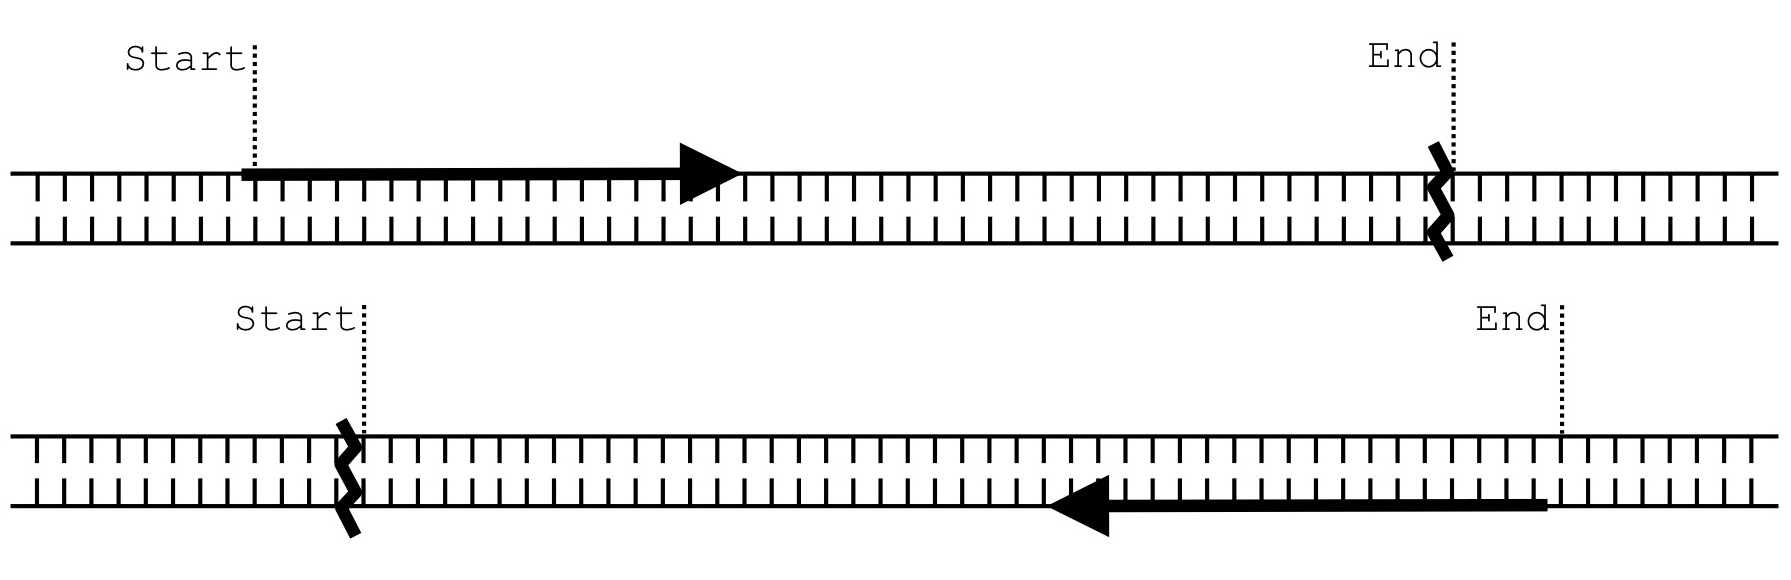
\includegraphics[width=\textwidth]{endogenous_breaksite}
\caption{\textbf{Endogenous breaksite} strategies are shown in the \texttt{+} strand orientation \textbf{(Top)} and \texttt{-} orientation \textbf{(Bottom)}. \texttt{Start} and \texttt{End} coordinates are marked. Diagrams are oriented so that chromosomal coordinates increase from left to right.}
\label{overflow}
\end{figure}

\subsection{Non-Endogenous Breaksite Libraries (Breaksite Cassette)}
\paragraph{} The annotation is marginally more complicated for non-endogenous breaksite libraries than for endogenous breaksites because the pipeline needs a little extra information about where the breaksite cassette has been inserted into the genome as well as what that sequence is. The \texttt{Breakseq} column contains the sequence of the entire cassette written from priming end to cutting end. The \texttt{Chr}, \texttt{Start}, \texttt{End}, and \texttt{Strand} columns together fully annotate the cassette position and direction. The \texttt{Strand} is the orientation of the cassette, either \texttt{+} or \texttt{-}, and is determined by the orientation of the primer. \emph{Note: regardless of the orientation, the breaksite cassette sequence must be given from priming end to cutting end.} Again, we will follow the convention of requiring the end coordinate to be greater than the start coordinate. To determine the \texttt{Start} column, find the last basepair coordinate of endogenous locus before the start of the cassette and add 1 to this number. The \texttt{End} column denotes the first basepair coordinate of endogenous locus after the end of the cassette.
\paragraph{} While in endogenous breaksite libraries the priming site is given explicitly, this is not so in non-endogenous breaksite libraries because the priming site can be determined using the primer sequence and the breaksite sequence. However, that still leaves one last piece of information to be accounted for in the non-endogenous breaksite libraries and that is the specific location of the cutting site. This coordinate is with respect to the sequence entered in \texttt{Breakseq} and is located in the \texttt{Breaksite} column.
\begin{figure}[ht]
\centering
  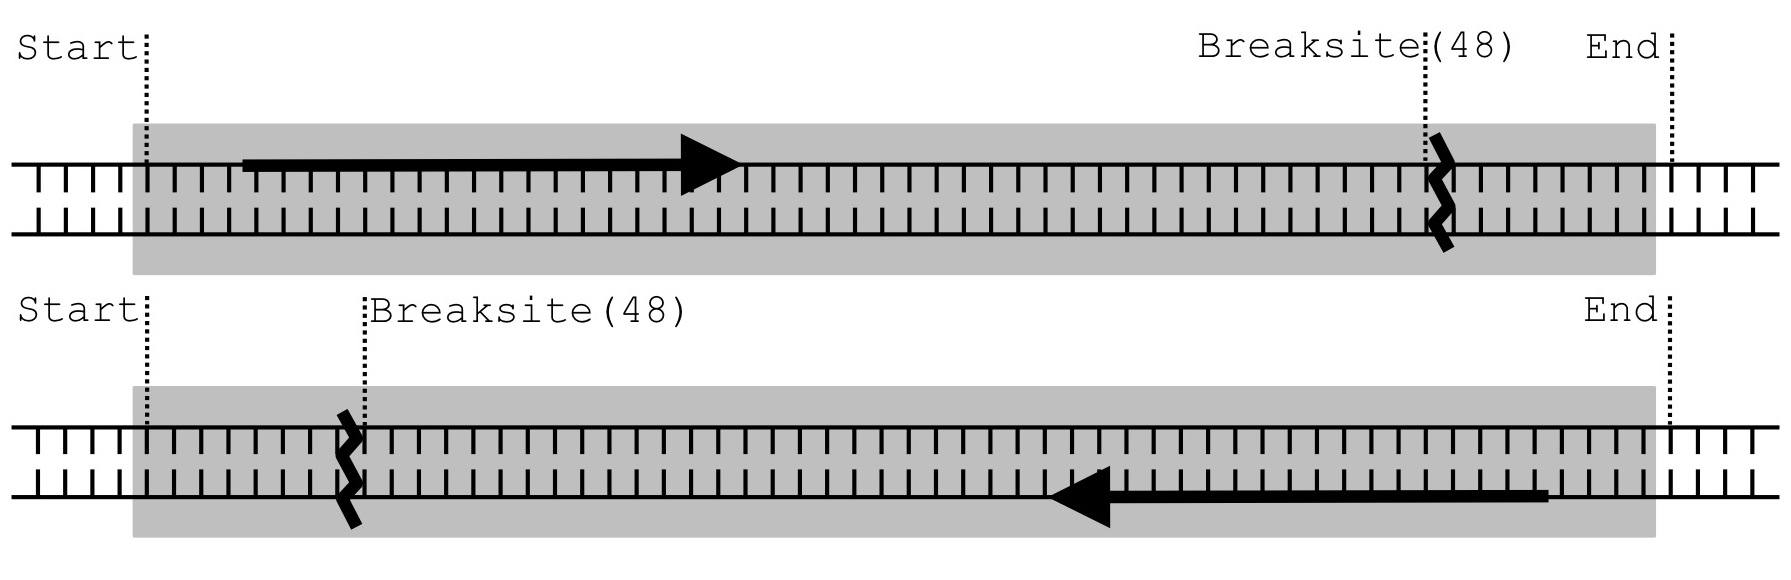
\includegraphics[width=\textwidth]{nonendogenous_breaksite}
\caption{\textbf{Non-endogenous breaksite} strategies are shown in the \texttt{+} strand orientation \textbf{(Top)} and \texttt{-} orientation \textbf{(Bottom)}. \texttt{Start} and \texttt{End} coordinates are marked. Diagrams are oriented so that chromosomal coordinates increase from left to right. The shaded area represents the non-endogenous cassette.}
\label{overflow}
\end{figure}




\end{document}